
Os dois jogos foram jogados pelo grupo em um PlayStation~5. As capturas foram extraídas das transmissões ao vivo feitas por um integrante do grupo no canal \textit{Nerd Geek TV}. Para cada jogo, a ficha traz os itens pedidos na análise: plataforma, situação de gameplay, momento, elemento visual, efeito, benefício e fonte técnica. Depois vêm as capturas marcadas e o vídeo.

Uma ressalva vale para os dois casos. Um jogo comercial não expõe seus shaders, e uma captura mostra só o resultado final. Quando o texto afirma como algo foi produzido, a afirmação vem de uma fonte do estúdio. Quando descreve um efeito observado na tela, ele é apresentado como \textit{compatível} com a técnica, e não como prova da implementação.

\textbf{Como ler as capturas.} Os retângulos amarelos numerados marcam onde o UV mapping está sendo aplicado. A legenda de cada figura explica cada número: qual técnica aparece e em qual equação do Capítulo~\ref{chap:equacoes} ela se encaixa.

\section{Rocket League}

\begin{table}[H]
\centering
\caption{Análise do Rocket League.}
\label{tab:ficha-rl}
\small
\begin{tabular}{p{3.0cm}p{11.0cm}}
\toprule
Jogo & \textit{Rocket League} (Psyonix), motor Unreal Engine~3 \cite{substance} \\
Plataforma & PlayStation~5, executando a versão de PS4 por retrocompatibilidade \cite{rlstore}, em 4K (\textit{checkerboard}) a 60 quadros por segundo com HDR \cite{rlps5} \\
Situação analisada & (a) Partida online e o \textit{replay} automático exibido após um gol; (b) tela inicial, com o carro do jogador em destaque \\
Momento & (a) Logo após o gol que deixou o placar em 4 a 3, faltando 3:18; (b) antes de entrar na partida \\
Elementos visuais & Carroceria, rodas e antena dos carros; bola; piso, faixas e painéis do estádio; rastro do \textit{boost} \\
Efeito produzido & Pinturas e decalques que seguem a forma de cada carro; piso e faixas repetidos em todo o campo; rastro animado atrás do carro ao acelerar \\
Benefício & O mesmo layout UV de cada carro recebe dezenas de pinturas, decalques e rodas, a base da personalização do jogo, sem novos modelos. As \textit{trim textures} reaproveitadas texturizam arenas inteiras com poucas imagens. O rastro animado dá retorno visual da aceleração sem geometria extra \\
Fonte técnica & Entrevista de um dos artistas líderes da Psyonix sobre o uso do Substance Designer no jogo \cite{substance} \\
\bottomrule
\end{tabular}
\end{table}

Segundo a entrevista \cite{substance}:
\begin{itemize}
    \item os mapas recentes foram texturizados inteiramente no Substance Designer, com \textit{trim textures} divididas em quartos para facilitar o UV mapping feito pelos modeladores;
    \item a banda de rodagem dos pneus e o relevo dos aros são gerados proceduralmente no Designer;
    \item um grafo combina mapas de curvatura e espessura com um mapa gerado a partir do layout UV de cada carro para criar os efeitos de borda dos decalques, e é reaplicado a cada carro novo;
    \item máscaras permitem aplicar a cor de cada time.
\end{itemize}
O rastro do \textit{boost} é o efeito em que se espera UV dinâmico: uma faixa animada que acompanha o carro. Em motores como a Unreal, esse tipo de efeito é montado com texturas em deslocamento, como as do nó \textit{Panner} \cite{unrealpanner}. Como o estúdio não detalha a implementação do rastro, e parte dele é feita de partículas (estrelas e fumaça, no item usado pelo jogador na live), ele é tratado aqui apenas como efeito compatível com a técnica.

\textbf{Cena da Figura~\ref{fig:rl-replay}.} Logo após um gol em partida online, o jogo exibe o \textit{replay} da jogada. A câmera acompanha a bola perto do gol, com o carro adversário (azul) e o do jogador (vermelho, marcado ``Você'') no fundo.

\begin{figure}[H]
    \centering
    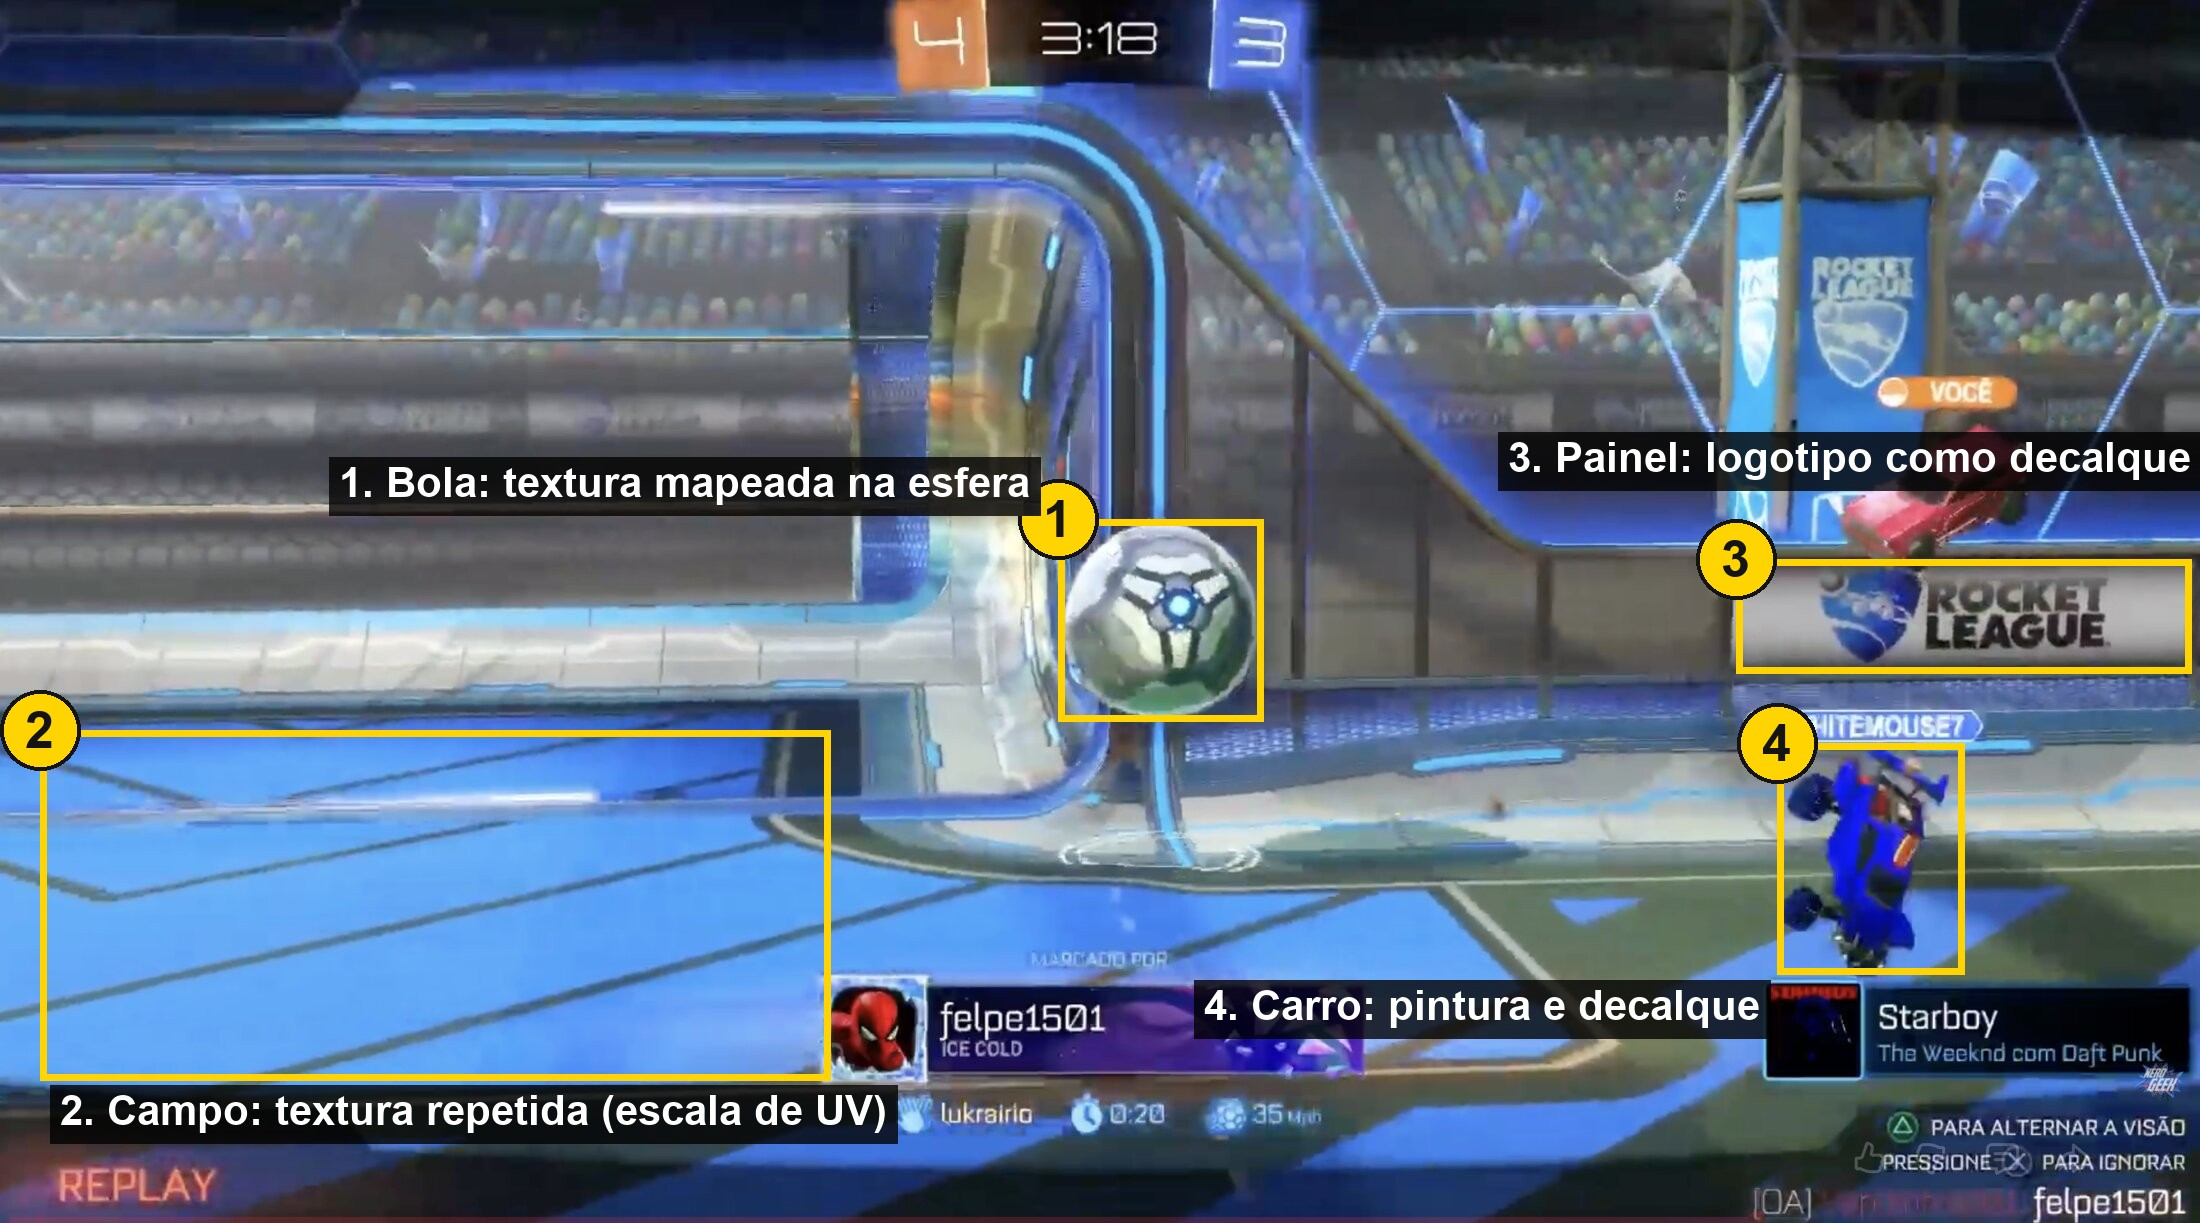
\includegraphics[width=0.92\textwidth]{imagens/marcadas/rl_replay.jpg}
    \caption{Rocket League (PS5), \textit{replay} após um gol. (1)~Bola: textura mapeada na esfera pelo UV. (2)~Campo: o piso e as faixas repetem a mesma textura, ladrilhamento por escala de UV (Eq.~\ref{eq:escala}). (3)~Painel com logotipo: decalque aplicado sobre a região UV do painel. (4)~Carro adversário: pintura sobre o UV do modelo.}
    \label{fig:rl-replay}
\end{figure}

\textbf{Cena da Figura~\ref{fig:rl-garagem}.} Na tela inicial, antes da partida, o jogo exibe o carro do jogador parado no gramado, com a pintura e as rodas escolhidas na garagem.

\begin{figure}[H]
    \centering
    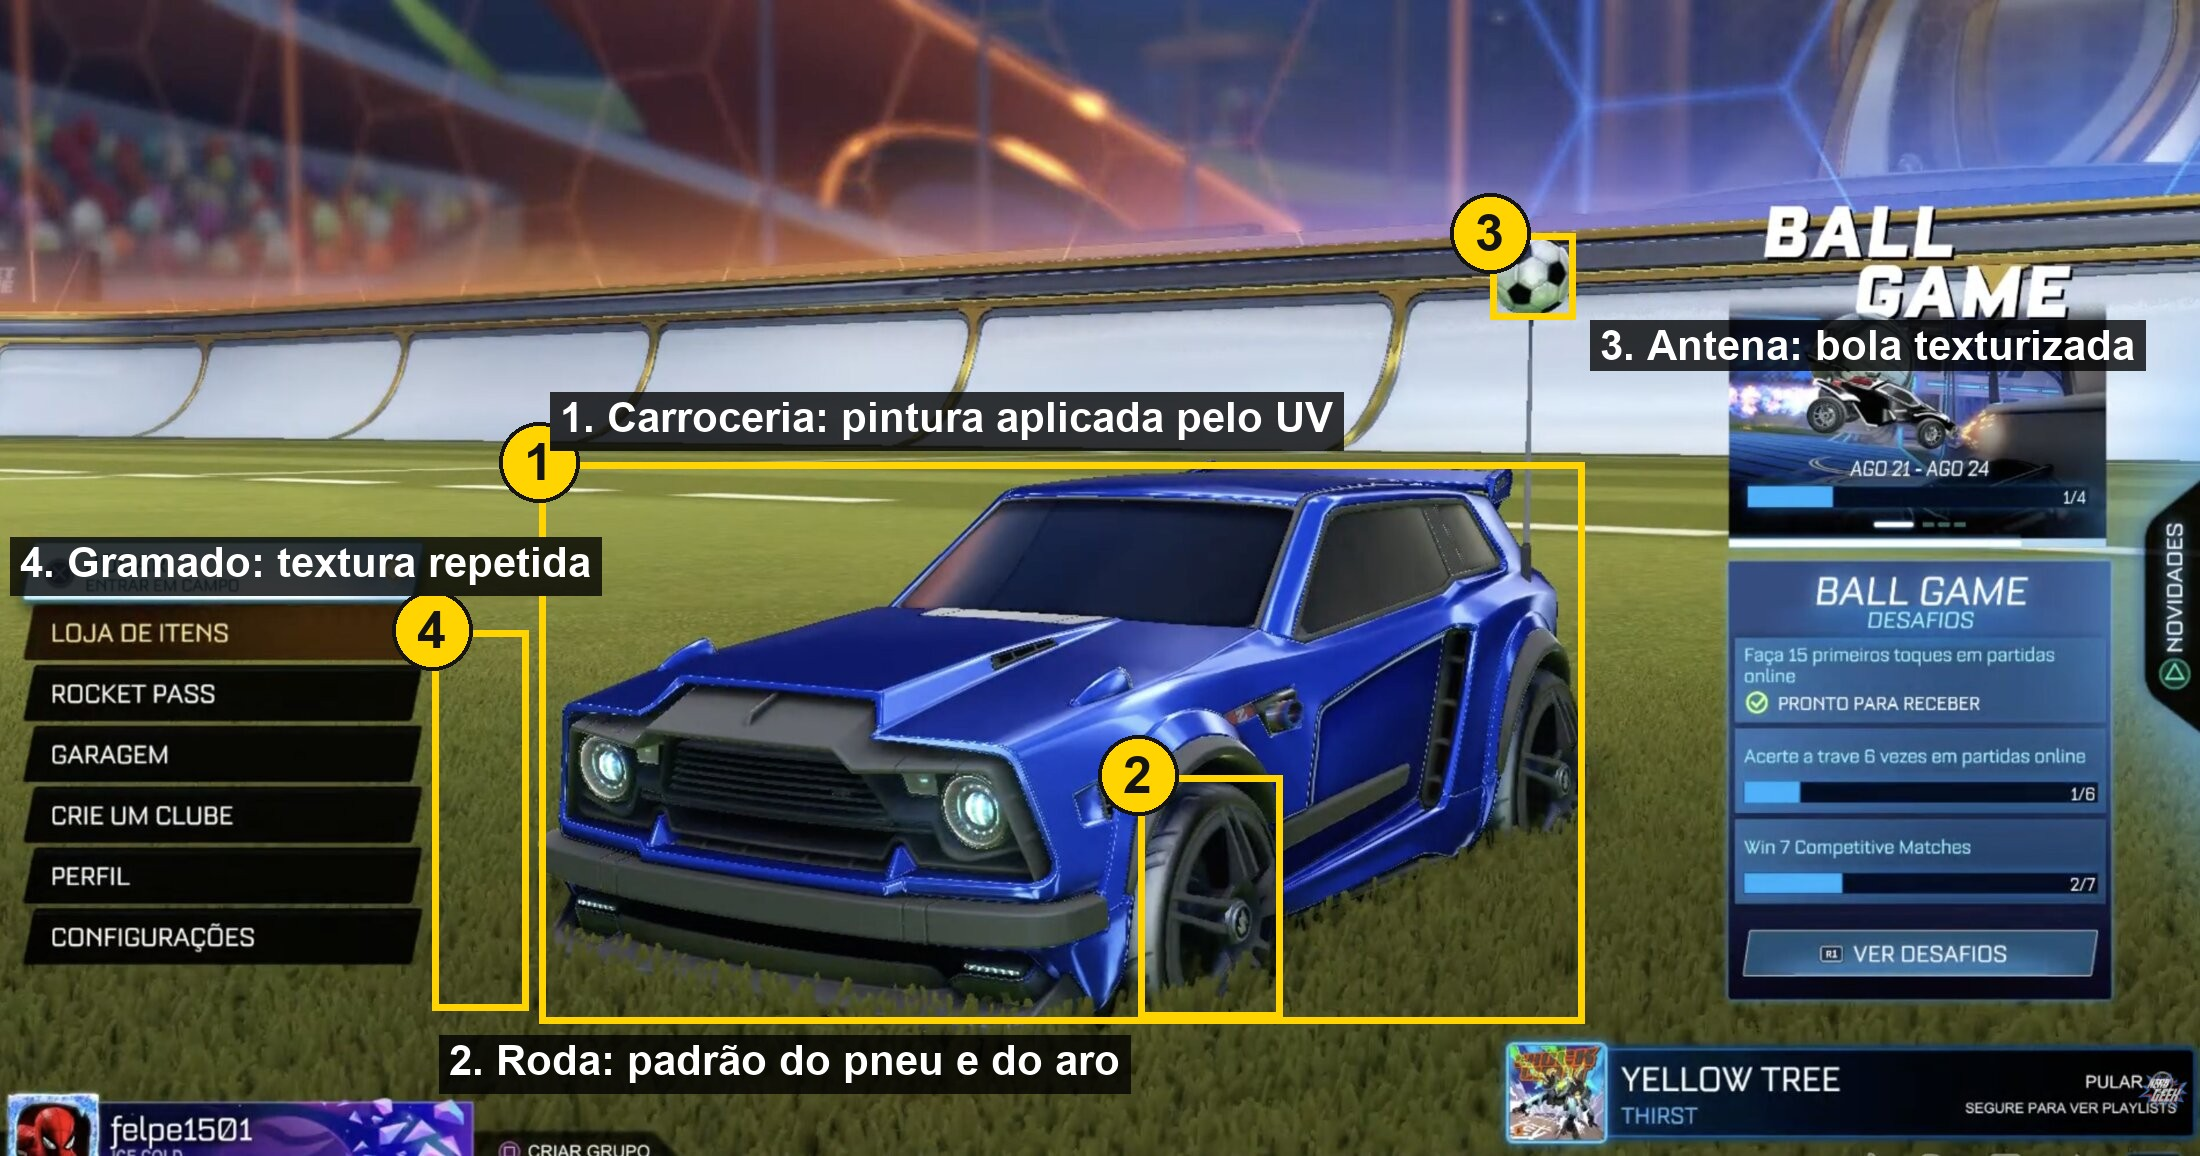
\includegraphics[width=0.92\textwidth]{imagens/marcadas/rl_garagem.jpg}
    \caption{Rocket League (PS5), tela inicial. (1)~Carroceria: a pintura é uma textura sobre o layout UV do carro; os decalques, quando equipados, usam o mesmo layout. (2)~Roda: banda de rodagem e aro gerados proceduralmente no Substance Designer \cite{substance}. (3)~Antena: esfera com textura própria. (4)~Gramado: textura repetida (Eq.~\ref{eq:escala}).}
    \label{fig:rl-garagem}
\end{figure}

\textbf{Vídeo.} Transmissão ao vivo do grupo (PS5): \url{https://www.youtube.com/live/eUX4mfkpFlQ}. Nela aparecem a tela inicial com o carro, os \textit{replays} após os gols e o rastro do \textit{boost} durante as partidas.

\section{Marvel's Spider-Man Remastered}

\begin{table}[H]
\centering
\caption{Análise do Marvel's Spider-Man Remastered.}
\label{tab:ficha-sm}
\small
\begin{tabular}{p{3.0cm}p{11.0cm}}
\toprule
Jogo & \textit{Marvel's Spider-Man Remastered} (Insomniac Games) \\
Plataforma & PlayStation~5, versão nativa, lançada em 12 de novembro de 2020 \cite{spidermanps} \\
Situação analisada & (a) Missão da história em que o Homem-Aranha observa um píer da polícia, em conversa por rádio com a ``Técnica da Torre''; (b) exploração livre no alto de um arranha-céu de Manhattan; (c) menu de pausa, aba \textit{Trajes} \\
Momento & (a) Durante a missão, com o personagem parado na borda do prédio; (b) no instante da notificação de desbloqueio do DLC ``A Cidade que Nunca Dorme''; (c) na escolha do traje \\
Elementos visuais & Fachadas dos prédios; traje do personagem; veículos e piso do píer; água da baía e dos rios \\
Efeito produzido & Janelas repetidas ao longo dos andares; padrão de teia acompanhando a curvatura do corpo; decalques sobre os veículos e o píer; superfície de água com textura de ondas \\
Benefício & As fachadas repetem um módulo de janela, o que permite texturizar uma cidade inteira com poucas imagens. Cada traje é um conjunto de texturas sobre o UV do personagem, o que permite oferecer dezenas de trajes \\
Fonte técnica & Página da Insomniac sobre a versão remasterizada (modelos e materiais melhorados, reflexos com \textit{ray tracing}) \cite{insomniac}. Para a água, a Insomniac não publica a implementação; o uso de UV em deslocamento é justificado pela técnica documentada nos motores \cite{unrealpanner,unitytiling} e demonstrado na implementação do grupo (Seção~\ref{sec:demo-app}) \\
\bottomrule
\end{tabular}
\end{table}

Neste jogo, a técnica aparece com mais clareza no UV tradicional: o padrão de teia dos trajes, os decalques dos veículos e as fachadas com janelas repetidas. A água da baía e dos rios é coberta por uma textura de ondas. Em jogos, superfícies de água desse tipo costumam ser animadas deslocando o UV da textura ao longo do tempo (Equações~\eqref{eq:translacao} e~\eqref{eq:onda}), em vez de deformar a geometria, como no nó \textit{Panner} \cite{unrealpanner}. Como a Insomniac não publica a implementação e uma captura estática não registra movimento, a água é tratada aqui apenas como efeito compatível com a técnica. A demonstração do UV dinâmico em funcionamento é feita na implementação do grupo (Seção~\ref{sec:demo-app}). Os reflexos sobre a água vêm de outra técnica, o \textit{ray tracing} \cite{insomniac}.

\textbf{Cena da Figura~\ref{fig:sm-pier}.} Durante uma missão, o Homem-Aranha está agachado na borda de um prédio, observando um píer com veículos da polícia, enquanto conversa por rádio com a ``Técnica da Torre''. A baía aparece ao fundo.

\begin{figure}[H]
    \centering
    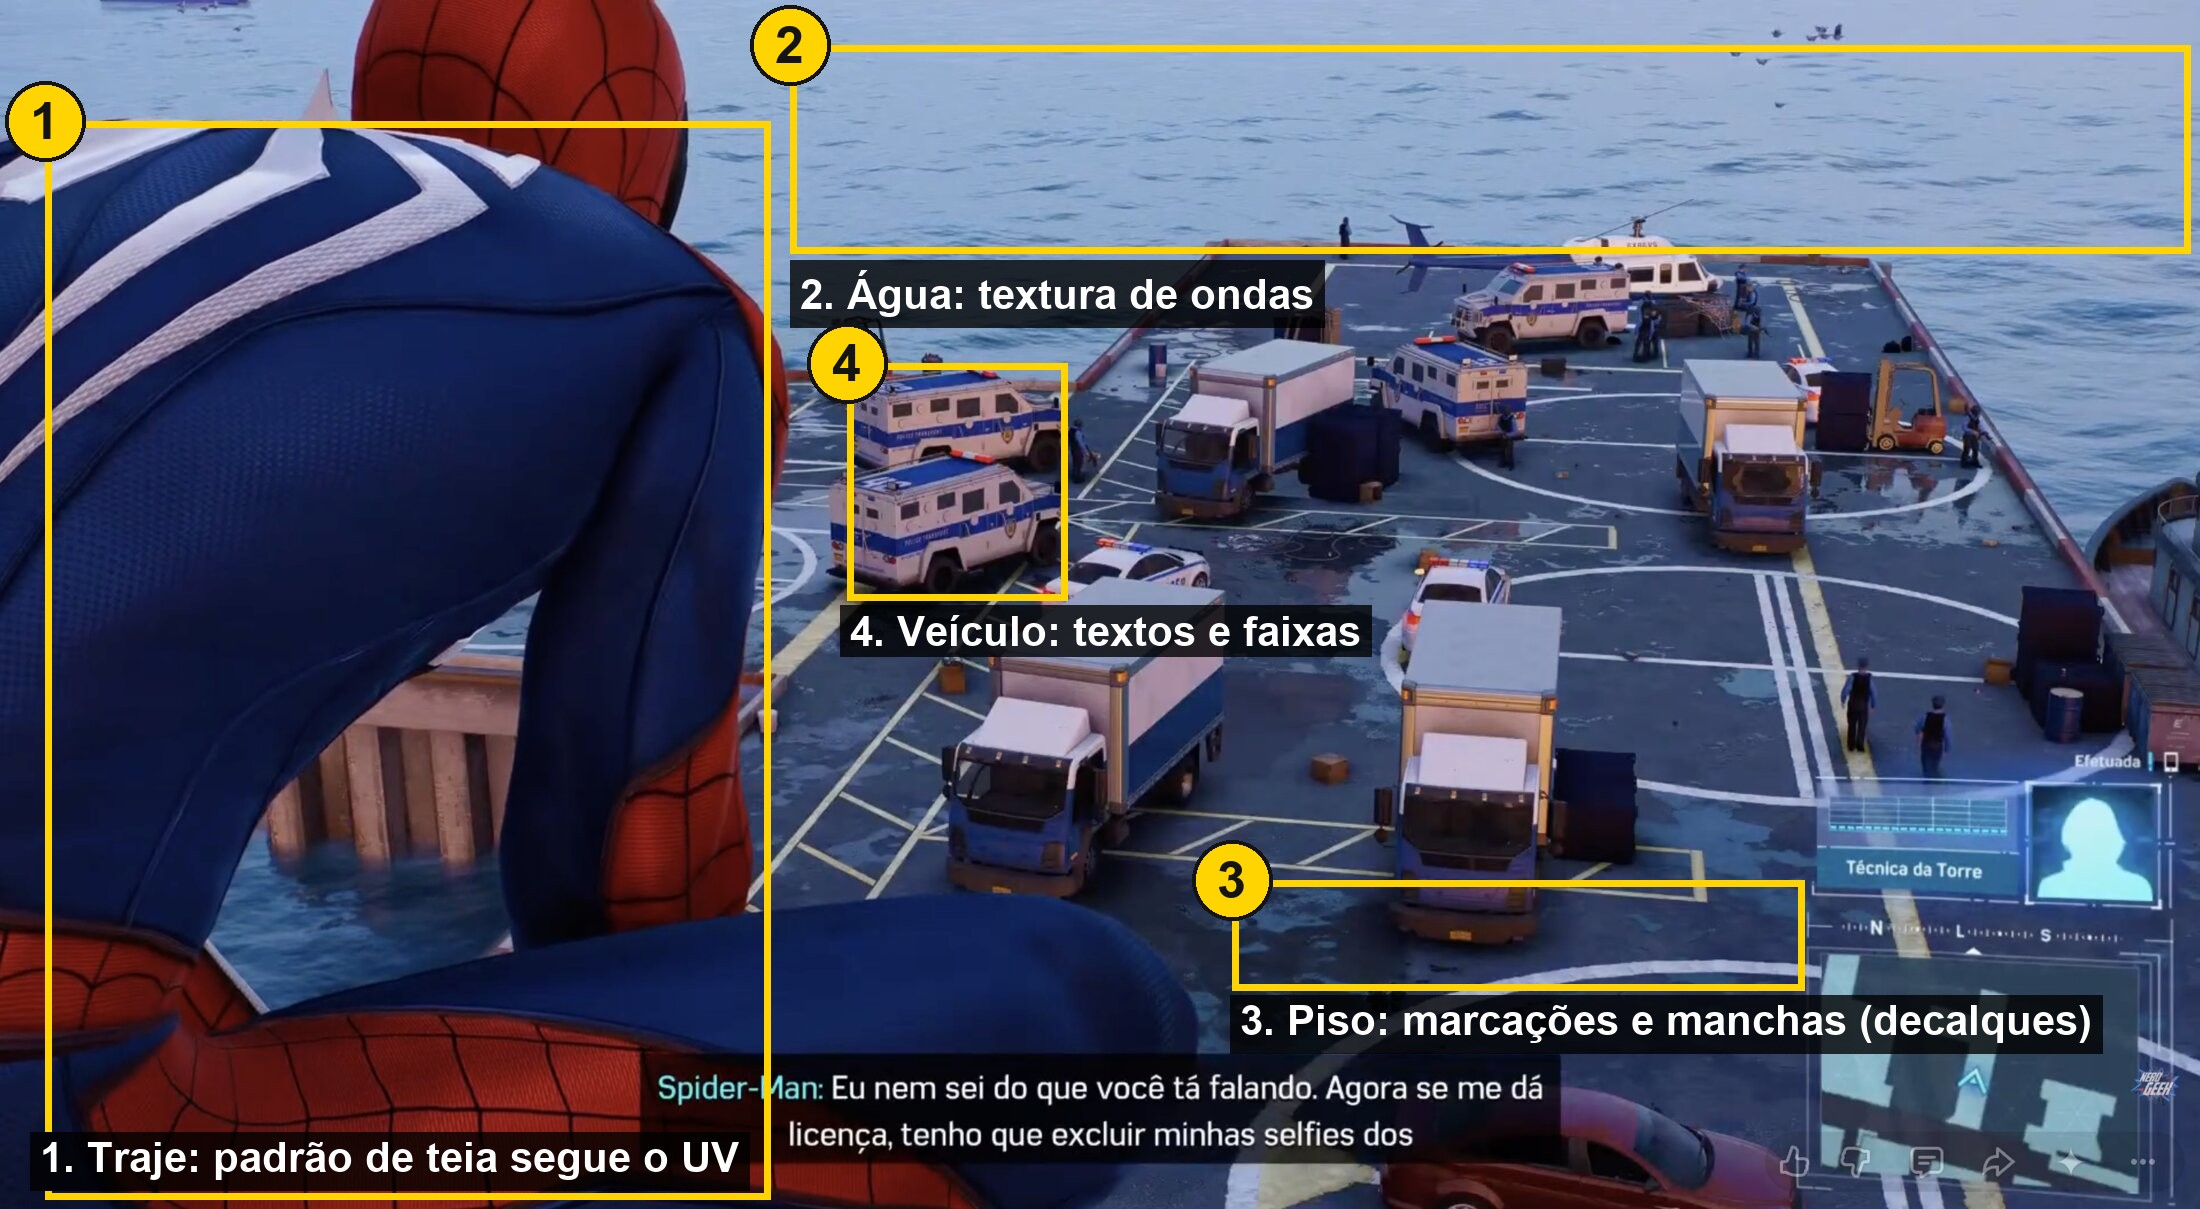
\includegraphics[width=0.92\textwidth]{imagens/marcadas/sm_pier.jpg}
    \caption{Marvel's Spider-Man Remastered (PS5), missão no píer da polícia. (1)~Traje: o padrão de teia e o relevo do tecido seguem o UV do personagem. (2)~Água: superfície coberta por uma textura de ondas; em jogos, esse tipo de superfície costuma ser animado deslocando o UV (Eqs.~\ref{eq:translacao} e~\ref{eq:onda}), o que uma imagem estática não permite confirmar. (3)~Piso do píer: marcações e manchas como decalques sobre uma textura repetida. (4)~Veículos: textos e faixas mapeados pelo UV de cada modelo.}
    \label{fig:sm-pier}
\end{figure}

\textbf{Cena da Figura~\ref{fig:sm-cidade}.} Na exploração livre, o personagem para no alto de um arranha-céu, com Manhattan e o rio à frente, no instante em que o jogo notifica o desbloqueio de um DLC.

\begin{figure}[H]
    \centering
    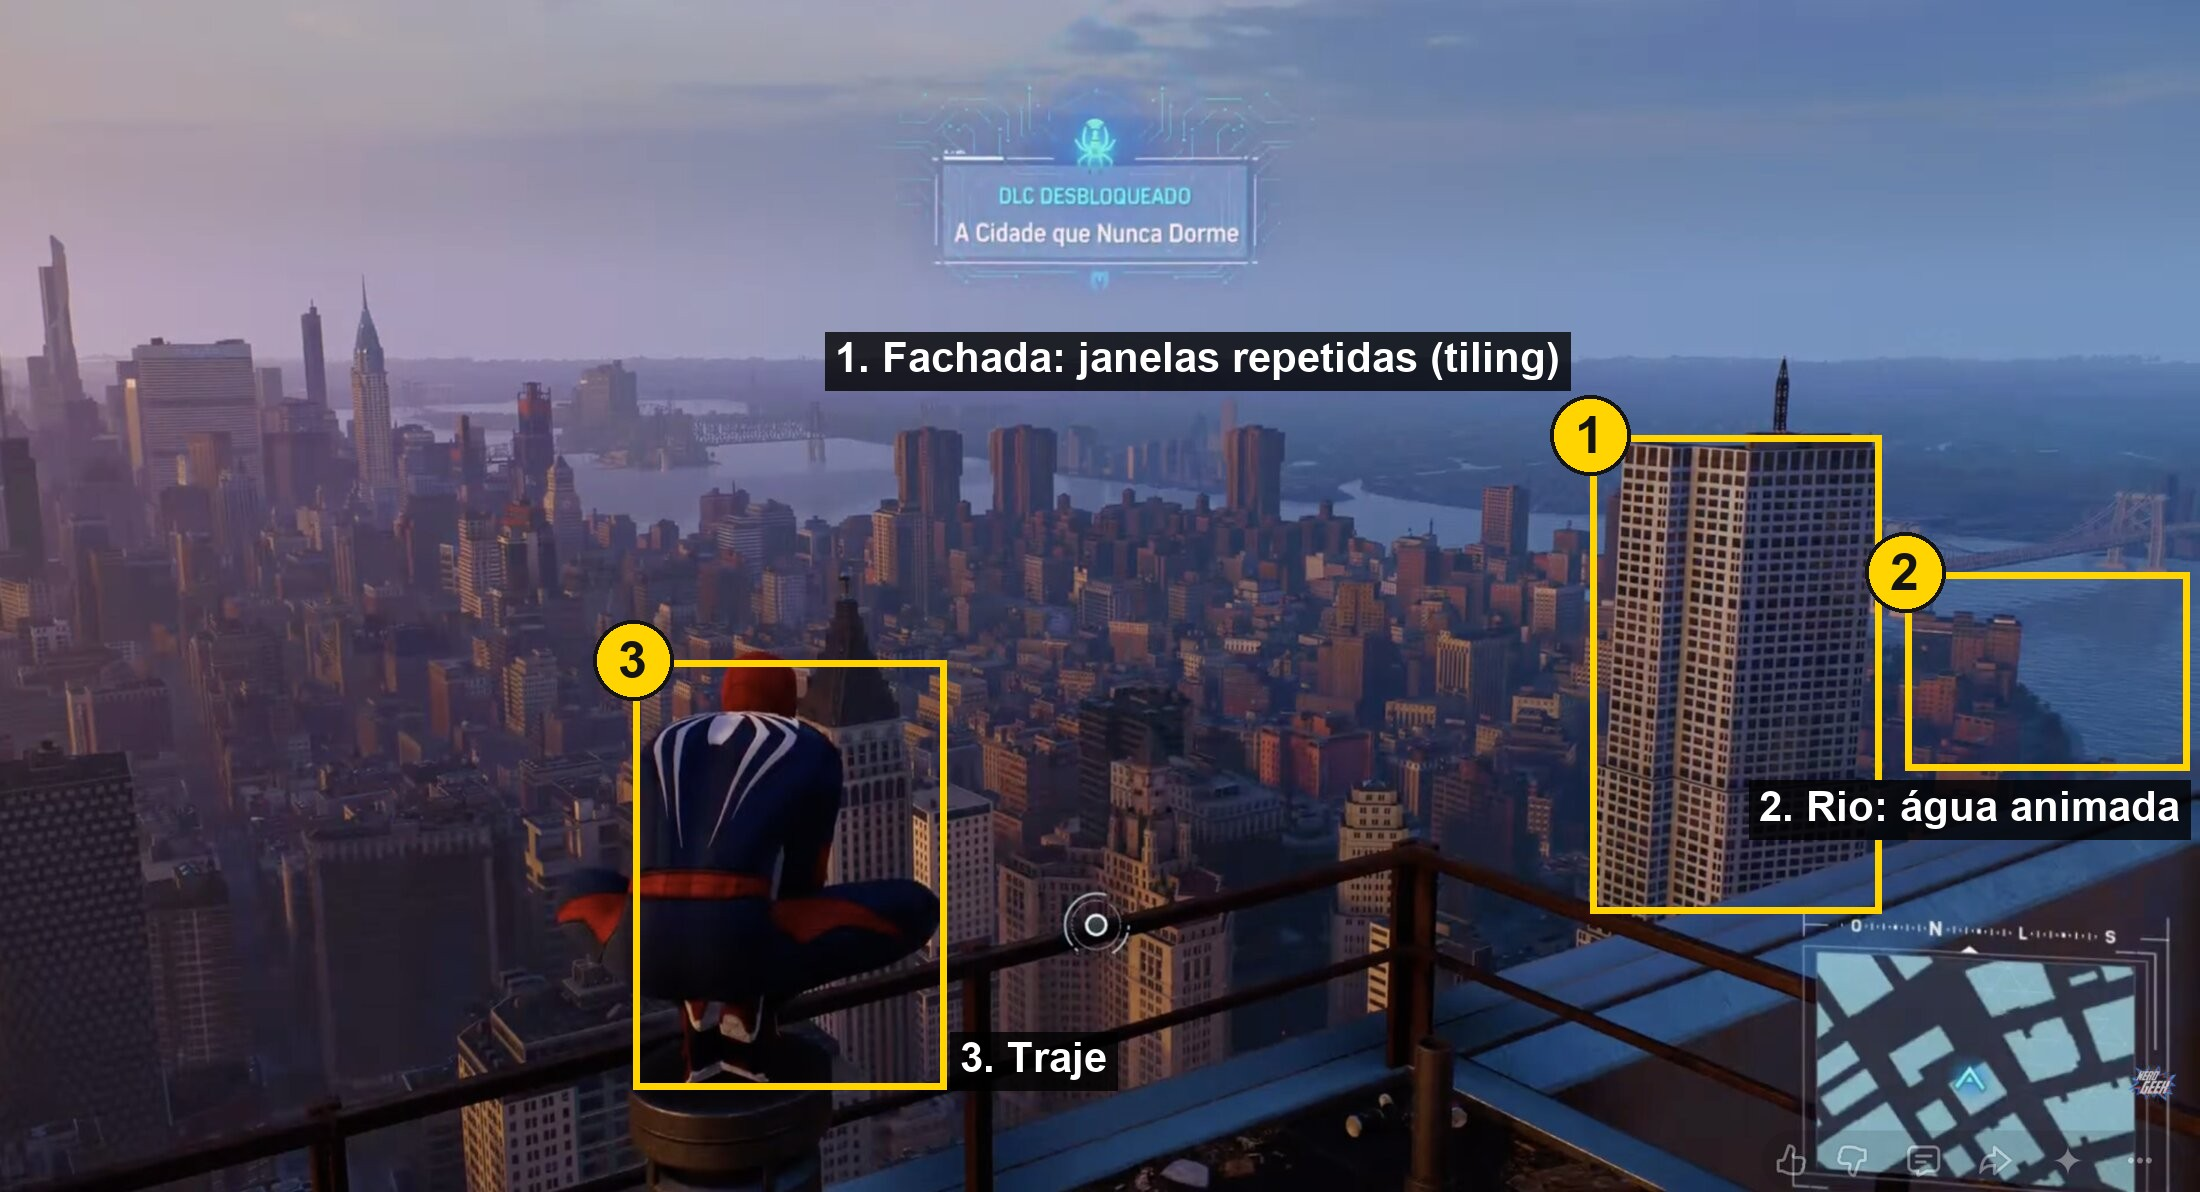
\includegraphics[width=0.92\textwidth]{imagens/marcadas/sm_cidade.jpg}
    \caption{Marvel's Spider-Man Remastered (PS5), exploração livre. (1)~Fachada: o mesmo módulo de janelas se repete ao longo dos andares (Eq.~\ref{eq:escala}). (2)~Rio: superfície de água com textura de ondas, a mesma da Figura~\ref{fig:sm-pier}. (3)~Traje do personagem, mapeado pelo UV.}
    \label{fig:sm-cidade}
\end{figure}

\textbf{Cena da Figura~\ref{fig:sm-trajes}.} No menu de pausa, aba \textit{Trajes}, o jogo exibe o modelo do personagem com o traje selecionado ao lado da lista de trajes desbloqueados.

\begin{figure}[H]
    \centering
    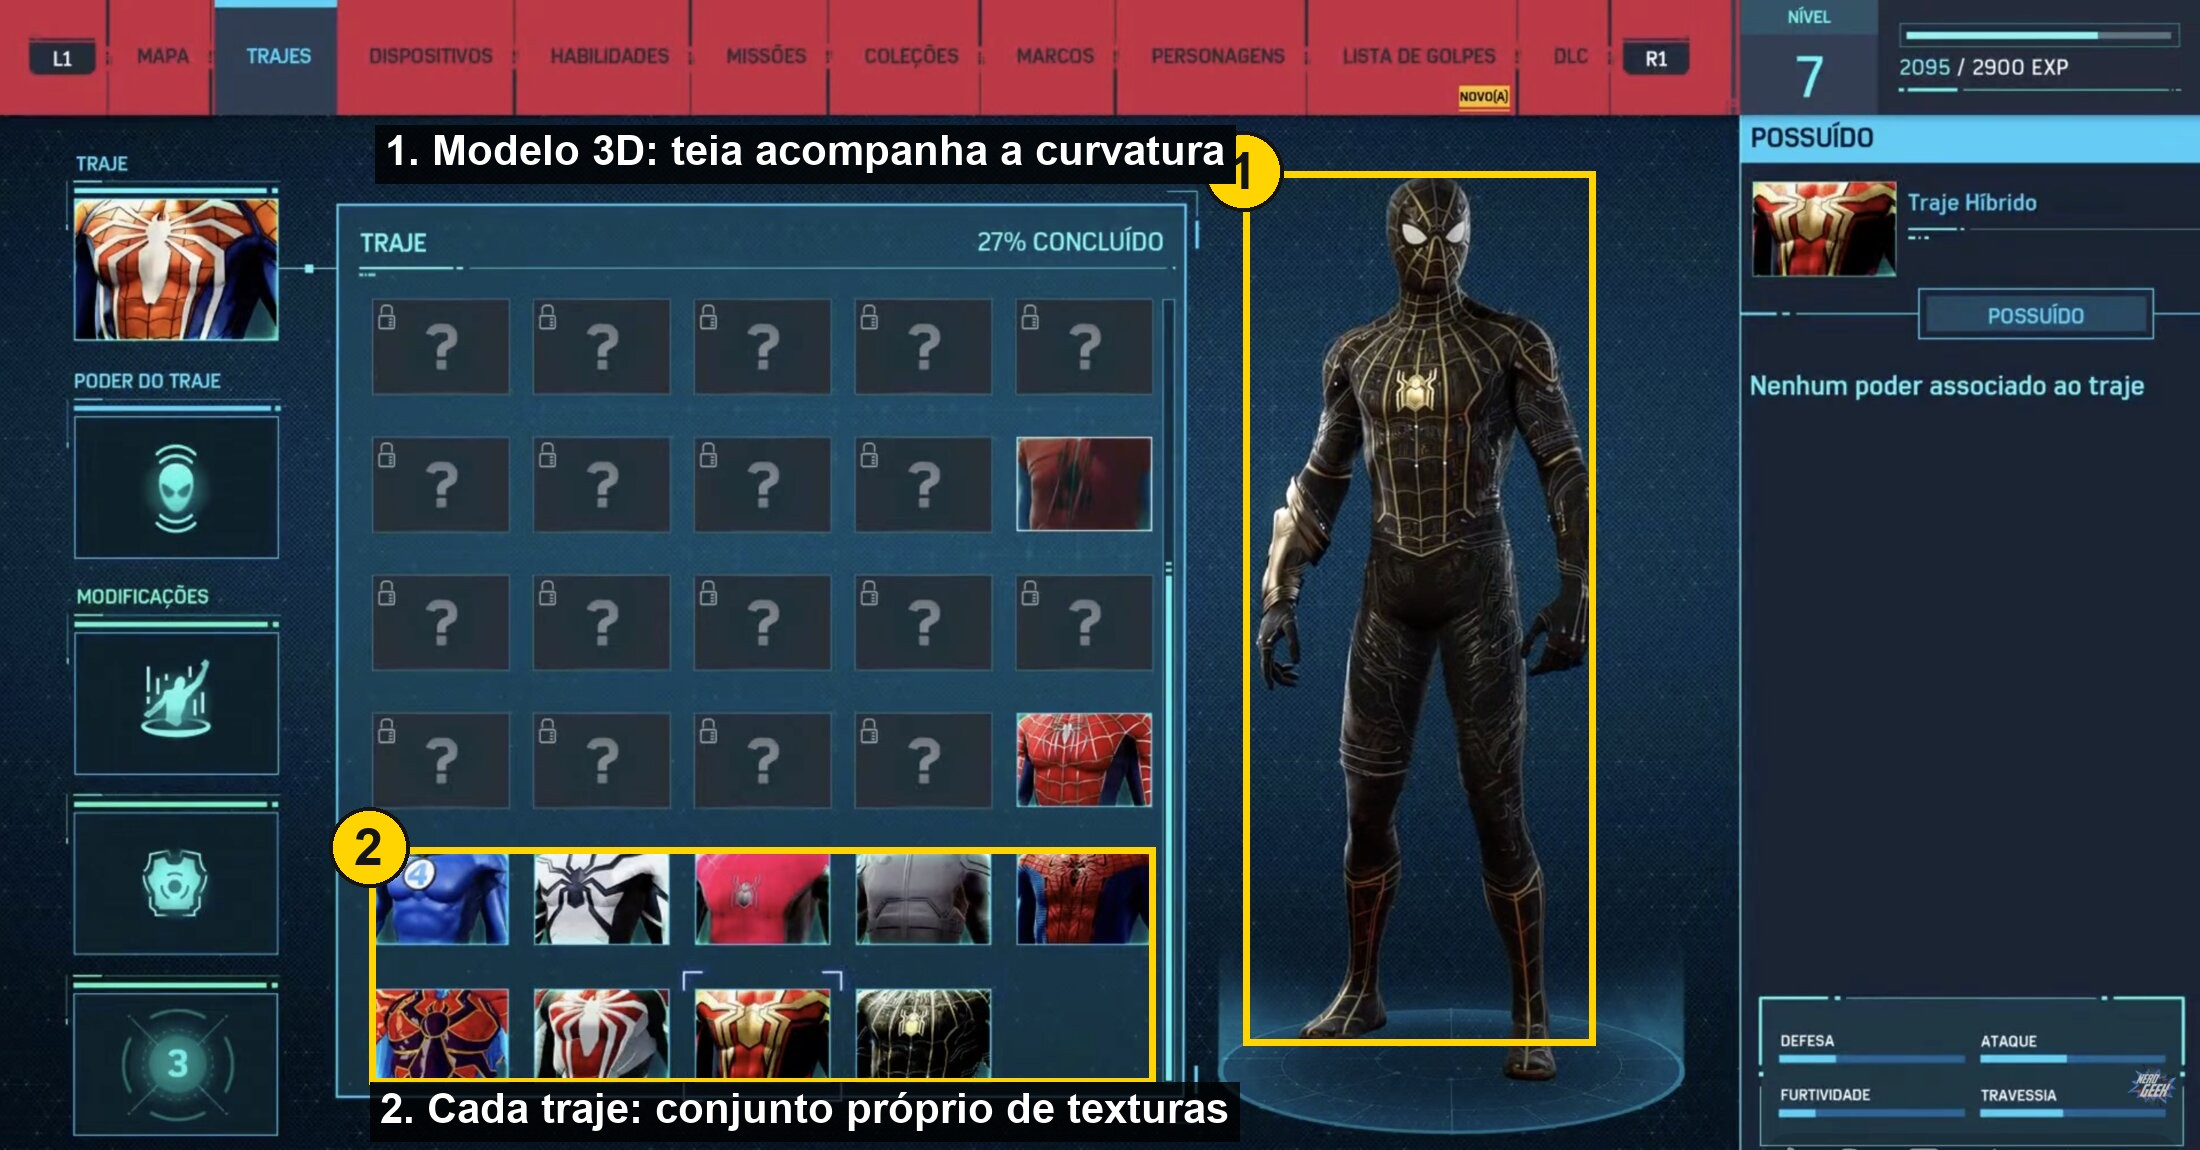
\includegraphics[width=0.92\textwidth]{imagens/marcadas/sm_trajes.jpg}
    \caption{Marvel's Spider-Man Remastered (PS5), menu de trajes. (1)~Modelo do personagem: as linhas da teia acompanham a curvatura do corpo, resultado da parametrização UV. (2)~Lista de trajes: cada traje é um conjunto próprio de texturas.}
    \label{fig:sm-trajes}
\end{figure}

\textbf{Lives completas.} Transmissões ao vivo do grupo (PS5): ``Parte 5'', \url{https://www.youtube.com/live/mhFPk9TQWWA}, e ``Parte 3'', \url{https://www.youtube.com/live/RKo-mqZgxG8}. Nelas aparecem as fachadas durante o balanço pela cidade, a baía e o menu de trajes.

\section{Demonstração na implementação do grupo}
\label{sec:demo-app}

Uma captura estática de um jogo comercial não registra movimento, e o código do jogo não está disponível. Por isso, a Figura~\ref{fig:app-uv-dinamico} demonstra o UV dinâmico na implementação Vulkan do grupo, em que ele pode ser comprovado quadro a quadro. A rotação do modelo foi pausada (tecla Espaço). O primeiro quadro está no modo~1, com a textura original, e os outros três estão no modo~2, com cerca de dois segundos de intervalo. A câmera e a malha não mudam entre os quadros. O olho, marcado com um círculo, começa na cabeça e atravessa o corpo à medida que \(u\) cresce com \(u' = u + 0{,}10\,t\) (Equação~\eqref{eq:translacao}).

\begin{figure}[H]
    \centering
    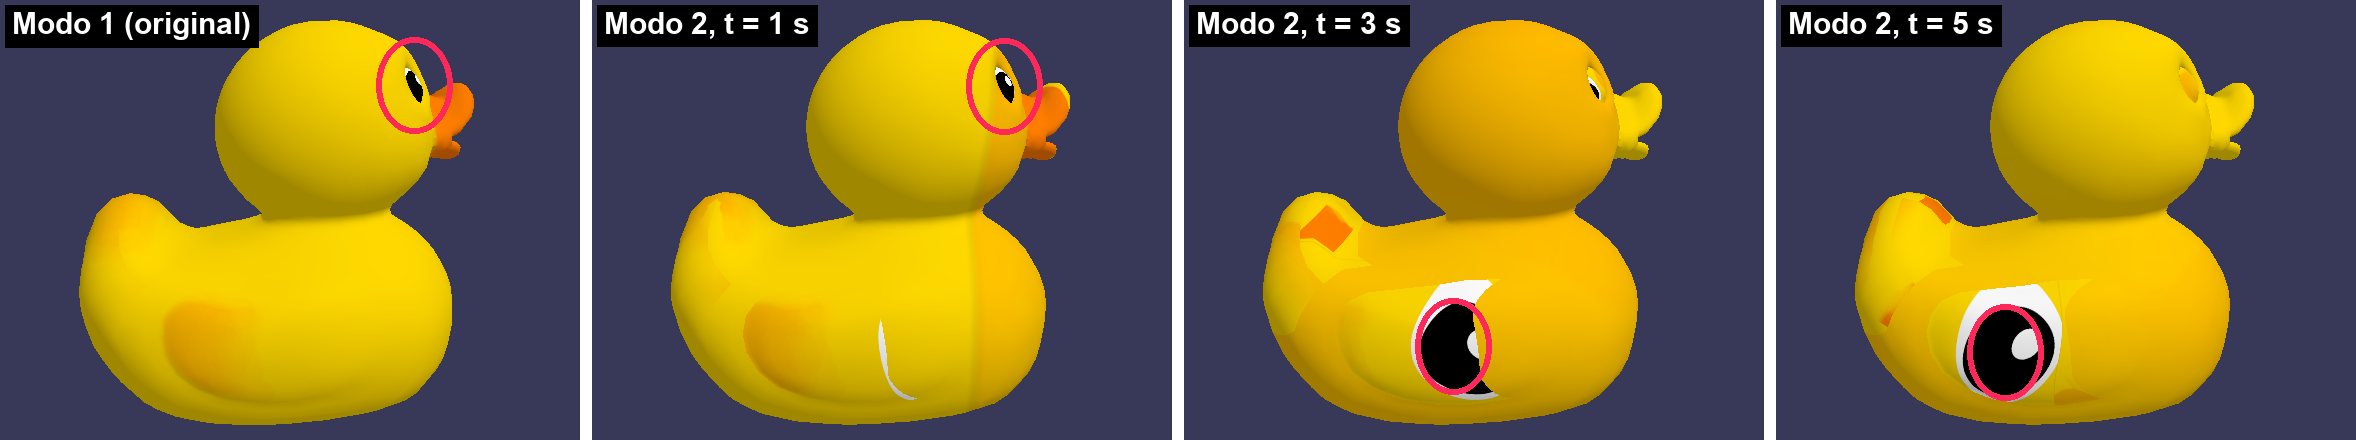
\includegraphics[width=\textwidth]{imagens/marcadas/app_uv_dinamico.png}
    \caption{Captura própria da implementação (Vulkan, \texttt{Duck.glb}): modo~1 e modo~2 em \(t \approx 1\), 3 e 5~s, com a malha parada. O olho (círculo) desliza da cabeça para o corpo porque o UV é deslocado no fragment shader (função \texttt{dynamicUV}).}
    \label{fig:app-uv-dinamico}
\end{figure}

\section{Comparação}

\begin{table}[H]
\centering
\caption{Técnicas observadas e onde aparecem nas capturas.}
\label{tab:marcacoes}
\small
\begin{tabular}{p{3.6cm}p{2.6cm}p{7.6cm}}
\toprule
\textbf{Técnica} & \textbf{Equação} & \textbf{Onde aparece} \\
\midrule
UV tradicional & \eqref{eq:uv}, \eqref{eq:perspectiva} & Fig.~\ref{fig:rl-replay}~(1, 4); Fig.~\ref{fig:rl-garagem}~(1, 3); Fig.~\ref{fig:sm-pier}~(1, 4); Fig.~\ref{fig:sm-cidade}~(3); Fig.~\ref{fig:sm-trajes}~(1, 2) \\
Ladrilhamento por escala & \eqref{eq:escala}, \eqref{eq:repeat} & Fig.~\ref{fig:rl-replay}~(2); Fig.~\ref{fig:rl-garagem}~(4); Fig.~\ref{fig:sm-cidade}~(1) \\
Decalque & \eqref{eq:uv} & Fig.~\ref{fig:rl-replay}~(3); Fig.~\ref{fig:sm-pier}~(3) \\
Procedural (na produção) & --- & Fig.~\ref{fig:rl-garagem}~(2): pneu e aro gerados no Substance Designer \cite{substance} \\
UV dinâmico & \eqref{eq:translacao}, \eqref{eq:onda} & Fig.~\ref{fig:app-uv-dinamico} (comprovado na implementação); Fig.~\ref{fig:sm-pier}~(2) e Fig.~\ref{fig:sm-cidade}~(2) (água, compatível); rastro do \textit{boost} no Rocket League (compatível) \\
\bottomrule
\end{tabular}
\end{table}

Nos dois jogos, o UV tradicional é o que viabiliza a escala do conteúdo: dezenas de carros e trajes personalizáveis e uma cidade inteira texturizada com módulos repetidos. O UV dinâmico é esperado onde o jogo precisa de movimento contínuo e barato: a água no Spider-Man e o rastro do \textit{boost} no Rocket League. Nos dois casos, porém, os estúdios não publicam a implementação, e o rastro do \textit{boost} ainda combina partículas (pequenas imagens que nascem e somem atrás do carro) com o brilho do rastro. Por isso, este trabalho trata esses efeitos como compatíveis com a técnica e demonstra o UV dinâmico em funcionamento na própria implementação (Figura~\ref{fig:app-uv-dinamico}), onde o deslocamento pode ser medido.
